\documentclass[12pt,letterpaper]{article}
\usepackage[utf8]{inputenc}
\usepackage[spanish]{babel}
\usepackage{graphicx}
\usepackage[left=2cm,right=2cm,top=2cm,bottom=2cm]{geometry}
\usepackage{graphicx} % figuras
% \usepackage{subfigure} % subfiguras
\usepackage{float} % para usar [H]
\usepackage{amsmath}
%\usepackage{txfonts}
\usepackage{stackrel} 
\usepackage{multirow}
\usepackage{enumerate} % enumerados
\renewcommand{\labelitemi}{$-$}
\renewcommand{\labelitemii}{$\cdot$}
% \author{}
% \title{Caratula}
\begin{document}

% Fancy Header and Footer
% \usepackage{fancyhdr}
% \pagestyle{fancy}
% \cfoot{}
% \rfoot{\thepage}
%

% \usepackage[hidelinks]{hyperref} % CREA HYPERVINCULOS EN INDICE

% \author{}
\title{Caratula}

\begin{titlepage}
\begin{center}
\large{UNIVERSIDAD PRIVADA DE TACNA}\\
\vspace*{-0.025in}
\begin{figure}[htb]
\begin{center}

\includegraphics[width=8cm]{./Imagenes/logo}
\end{center}
\end{figure}
\vspace*{0.15in}
INGENIERIA DE SISTEMAS  \\

\vspace*{0.5in}
\begin{large}
TITULO:\\
\end{large}

\vspace*{0.1in}
\begin{Large}
\textbf{INFORME DE LABORATORIO No 01} \\
\end{Large}

\vspace*{0.3in}
\begin{Large}
\textbf{CURSO:} \\
\end{Large}

\vspace*{0.1in}
\begin{large}
INTELIGENCIA DE NEGOCIOS\\
\end{large}

\vspace*{0.3in}
\begin{Large}
\textbf{DOCENTE(ING):} \\
\end{Large}

\vspace*{0.1in}
\begin{large}
 Patrick Cuadros Quiroga\\
\end{large}

\vspace*{0.2in}
\vspace*{0.1in}
\begin{large}
Integrantes: \\
\begin{flushleft}


Mamani Ayala  Brandon \hfill  (2015052715) \\
Ordoñez Quilli Ronald 	\hfill  (2015052821) \\
Quispe Mamani Angelo        \hfill	(2015052826) \\
Vizcarra Llanque Jhordy        \hfill	(2015052719) \\
\end{flushleft}
\end{large}
\end{center}

\end{titlepage}


\tableofcontents % INDICE
\thispagestyle{empty} % INDICE SIN NUMERO
\newpage
\setcounter{page}{1} % REINICIAR CONTADOR DE PAGINAS DESPUES DEL INDICE

\section{Actividad No 01 – Manipulaci\'on de Datos} 

\begin{enumerate}[1.]
	\item El departamento de Recursos Humanos requiere crear sentencias SQL para insertar, actualizar y eliminar datos de empleados. Como prueba se utilizará la tabla Mis\_Empleados antes de remitir las sentencias al departamento de Recursos Humanos.

	\item Crear la tabla Mis\_Empleados utilizando la siguiente estructura.
	\begin{center}
	\includegraphics[width=8cm]{./Imagenes/imagen0102} 
	\end{center}
	\item Generar una sentencia de inserción de datos que permita añadir los siguientes registros:
	\begin{center}
	\includegraphics[width=8cm]{./Imagenes/imagen0103} 
	\end{center}

	\item Generar un script que permita que mediante utilización de variables de sustitución, la inserción de información en la tabla Mis\_Empleados.

	\item Utilizando el script anterior adicionar los siguientes registros.
	\begin{center}
	\includegraphics[width=5cm]{./Imagenes/imagen0105} 
	\end{center}
	\item Revisar los cambios hechos a la tabla.
	\item Cambiar el nombre del empleado No 3 a Benjamín.
	\item Elevar el salario a \$ 1,000 a todos los empleados que tengan un salario menor a esa cantidad.
	\item Eliminar el registro del empleado María Castro
	\item Revisar los cambios hechos a la tabla.
	\item Confirmar los cambios a la tabla.
	\item Adicionar el siguiente registro a la tabla
	\\exec insertar\_datos 6,'Hurtado Gamboa','Ernesto','ehurtado',1400
	\\ go
	\item Revisar la adición realizada
	\item Crear un punto de restauración intermedio para esta transacción
	\item Borrar los registros de la tabla MIS\_EMPLEADOS.
	\item Revisar los cambios realizados.
	\item Descartar los cambios hechos a la tabla sin descartar la última adición hecha.
	\item Revisar nuevamente los registros de la tabla MIS\_EMPLEADOS.
	\item Confirmar todos los cambios hechos a la tabla MIS\_EMPLEADOS.
	\item Modificar el script del punto 4.4. a fin de que se genere automáticamente el CODIGO del empleado que lo conforman la primera letra de su nombre y la primera palabra de su apellido.
	\item Adicionar el siguiente registro a la tabla a fin de corroborar el funcionamiento del script anterior
           \\exec insertar\_datos 7,'Valdivia Pérez','Graciela',1800;
           \\go
	\item Revisar los cambios realizados. Y finalmente confirmar todos los cambios hechos a la tabla MIS\_EMPLEADOS.
\end{enumerate} 

\section{INTRODUCCION} 

En los \'ultimos años, las organizaciones han recurrido cada vez mas a soluciones de software avanzadas para administrar las cargas de trabajo, mantener la rentabilidad y asegurar la competitividad dentro de sus respectivas industrias. Si bien hay varias opciones disponibles, las herramientas de inteligencia de negocios (BI) y las herramientas de an\'alisis de negocios (BA) son posiblemente las soluciones de administraci\'on de datos mas implementadas. Los analistas de negocios y los compradores de software a menudo preguntan cuáles son las diferencias clave entre la inteligencia de negocios y los análisis de negocios.

Las soluciones de inteligencia empresarial se encuentran entre las herramientas de administraci\'on de datos mas valiosas disponibles. Las soluciones de BI recopilan y analizan datos actuales y procesables con el fin de proporcionar información para mejorar las operaciones comerciales. ¿Est\'a buscando formas de entender mejor sus operaciones comerciales? ¿Qu\'e hay de descubrir puntos de dolor en sus flujos de trabajo? ¿Qu\'e hay de analizar grandes conjuntos de datos para obtener información valiosa? Necesita una solución de inteligencia de negocios.

El software de an\'alisis de negocios es un niño o padre (dependiendo de a qui\'en le pregunte) de la categor\'ia de inteligencia empresarial. Al igual que BI, se utiliza principalmente para analizar datos hist\'oricos, pero con la intención de predecir las tendencias de negocios. Por lo general, también tiene un ojo hacia la mejora y la preparación para el cambio.
\section{MARCO TEORICO} 
		
\begin{enumerate}[1.]
	\item Business Analytics :
\\
\\
Al igual que la inteligencia de negocios, BA recopila y analiza datos, emplea análisis predictivos y genera informes visualizados en paneles personalizados. El objetivo de estas características es ayudar a identificar y abordar los puntos débiles de una organización. Aquí es donde terminan las similitudes. El software de análisis de negocios se utiliza para explorar y analizar datos históricos y actuales. Utiliza el análisis estadístico, la extracción de datos y el análisis cuantitativo para identificar las tendencias comerciales anteriores.
\\
Una vez que se han recopilado y analizado los datos, los sistemas de análisis de inteligencia empresarial los utilizan para el modelado predictivo. Esto puede predecir y, en la mayoría de los casos, prepararse para futuros climas empresariales. Uno de los aspectos más poderosos de BA es el informe ad-hoc, que permite a las empresas realizar análisis de datos específicos en tiempo real para responder preguntas específicas para tomar decisiones comerciales más rápidas. En efecto, el análisis de negocios utiliza el análisis predictivo para resolver problemas antes de que hayan ocurrido.

\end{enumerate}

\begin{center}
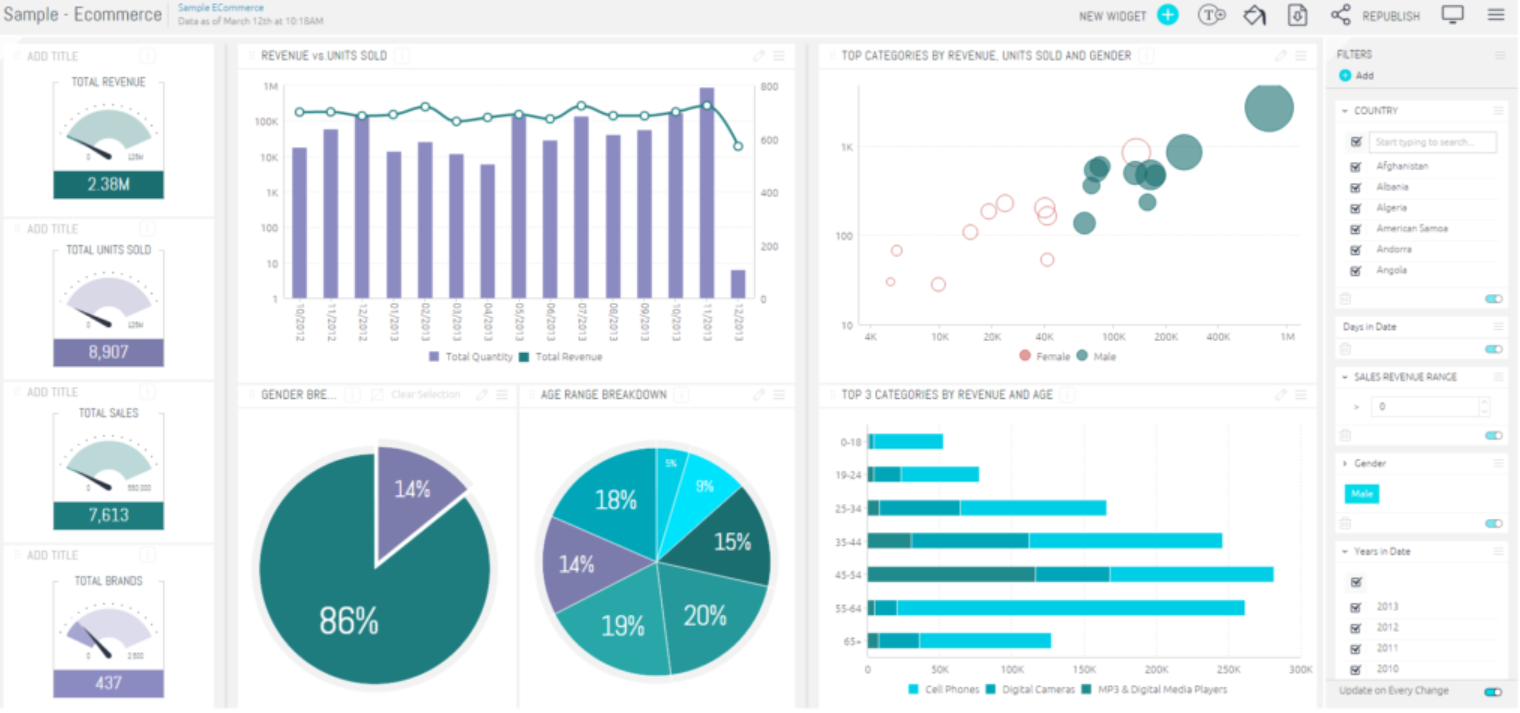
\includegraphics[scale=0.55]{./Imagenes/BA.png}
\end{center}



\end{document}
